\section{Implementierung}
In diesem Abschnitt befassen wir uns mit den wesentliche Implementierungs\-/Details
der zu dieser Arbeit begleitenden Software. Für die Implementierung wurde
die Programmiersprache C++ gewählt. Aufgrund der hohen effizienz von C++, ist die Sprache
gut geeignet für diese Art von Problem.

\subsection{Überblick}
 TODO diagramm?
\subsection{Verwendete Bibliotheken}
Es wurden drei externe Bibliotheken neben der STL verwendet:
\begin{enumerate}
    \item CLI11 \cite{cl11}\\
    Für den leichten Umgang mit Terminal\-/Eingaben.
    \item Eigen \cite{eigen}\\
    Zum Rechnen mit Matrizen und zur Lösung der Eigenwertsgleichungen.
    \item OpenMP \cite{omp}\\
    Zur Parallelsierung der Integralberechnung.
\end{enumerate}

\subsection{Atomorbitale und Basis\-/funktionen}\label{basis-functions-section}
Wir befassen uns nun genauer mit den verwendeten Atomorbitalen.
Wie am Anfang des letzten Kapitels beschrieben, werden Atomorbitale verwendet,
um die Molekülorbitale darzustellen. In diesem Kontext werden die Atomorbitale
Basisfunktionen genannt und die Menge der verwendeten Basisfunktionen
ist der so genannte Basis\-/Satz.
Die Basisfunktionen müssen jedoch nicht auf Atomorbitale beschränkt sein.
\cite[Ab. 5.3.1]{lewars_2016}

Es werden üblicherweise zwei Arten von Basisfunktionen verwendet,
um Atomorbitale zu konstruieren:

\begin{enumerate}
    \item Slater-Type-Orbitals (STO)\\
    STOs werden durch die analytischen Lösungen des Wasserstoff\-/Atoms dargestellt
    und können deshalb die Wellenfunktionen von Atomen sehr genau repräsentieren.
    Jedoch fällt die Berechnung der 2\-/Elektronen\-/Integrale schwer,
    weshalb die Verwendung von so genannten GTOs bevorzugt wird.

    \cite[Ab. 5.2]{cramer_2004}
    \cite[S. 2]{tc2_6}

    \item Gaussian-Type-Orbitals (GTO)\\
    Wie der Name schon bereits sagt, werden Gaussfunktionen verwendet,
    um die genaueren STOs zu approximieren. Im Gegensatz zu den STOs ist
    die Evaluierung der 2\-/Elektronen\-/Integrale mit GTOs viel leichter.
    GTOs werden durch die folgende kartesische Form definiert:\\
    \begin{equation}\label{gto-function}
        \chi(x,y,z) = N \cdot x^i y^j z^k \cdot \exp (-\alpha (x^2+y^2+z^2))
    \end{equation}

    Die Parameter $i,j,k$ entscheiden über die Art und Form des Orbitals (S, P, D ...).
    Die restlichen Parameter $N, \alpha$ dienen der Normierung und Anpassung der Größe des Orbitals.

    \begin{figure}[H]
        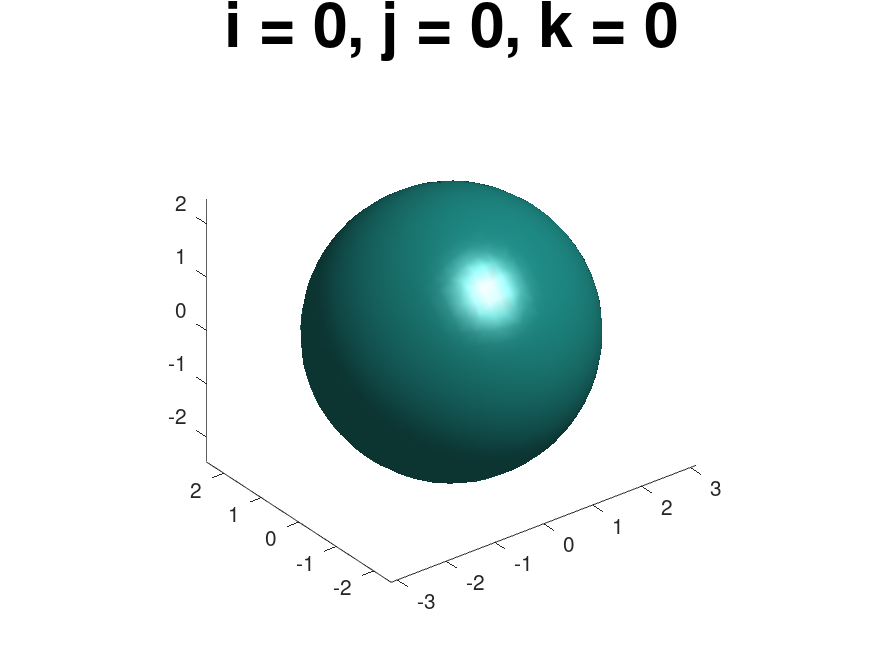
\includegraphics[trim=50 0 50 0, clip, width=0.24\textwidth]{res/GTOs/ao_0_0_0.png}
        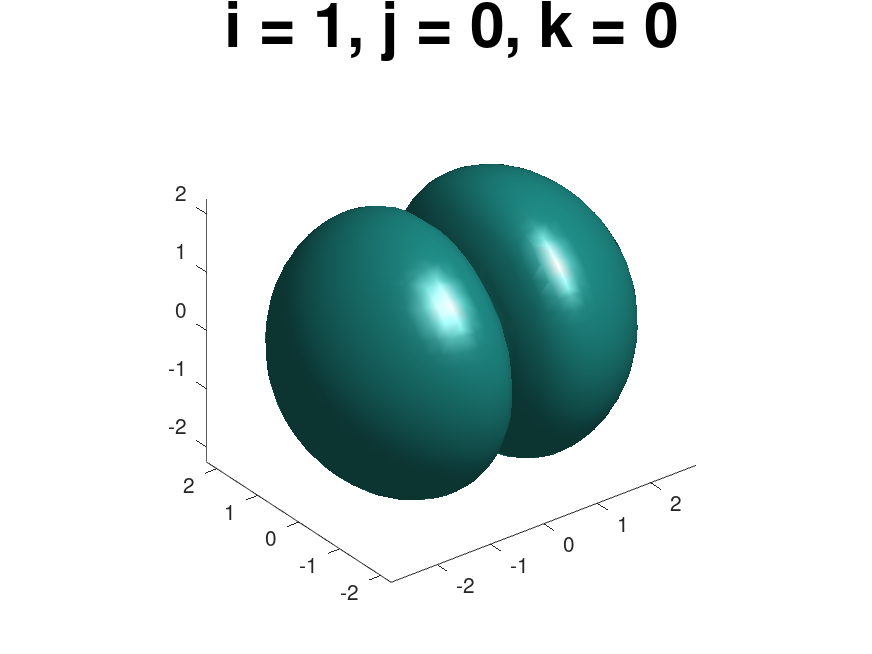
\includegraphics[trim=50 0 50 0, clip, width=0.24\textwidth]{res/GTOs/ao_1_0_0.png}
        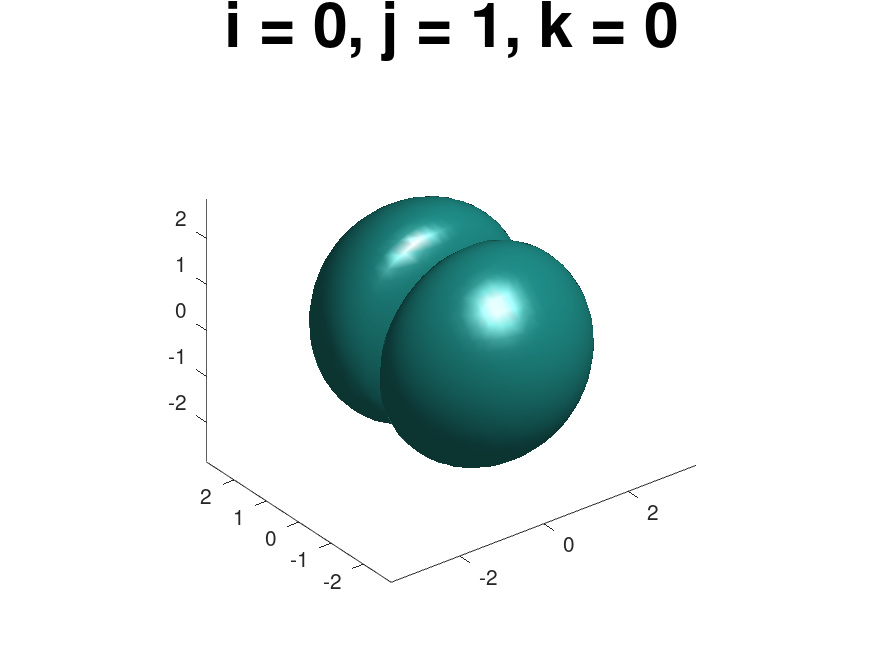
\includegraphics[trim=50 0 50 0, clip, width=0.24\textwidth]{res/GTOs/ao_0_1_0.png}
        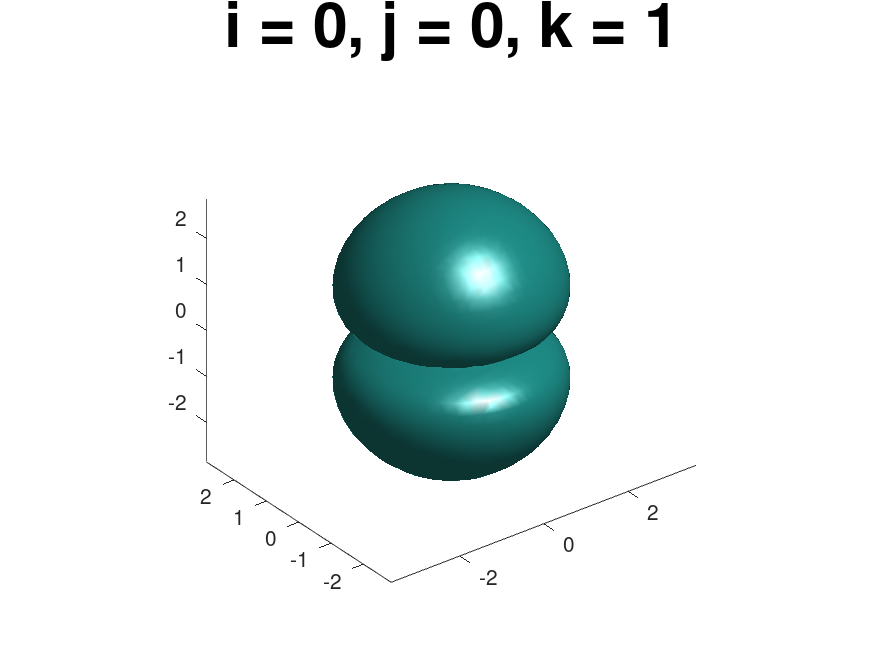
\includegraphics[trim=50 0 50 0, clip, width=0.24\textwidth]{res/GTOs/ao_0_0_1.png}
        \caption{GTOs des S-Orbitals und der drei P-Orbitale mit $N=2$ und $\alpha = 0.5$}
    \end{figure}

    \cite[Ab. 6.2.1]{cramer_2004}
\end{enumerate}

Der wesentliche Unterschied zwischen STOs und GTOs ist der radiale Zerfall,
welcher bei GTOs einer Gaussfunktion entspricht.
Diese Änderung ermöglicht ein exaktes Lösen der 2-Elektronen-Integrale,
die mit STOs nur numerisch genähert werden können.\cite[6.2.1]{cramer_2004}

In der Implementierung werden GTOs verwendet, aufgrund der leichteren Integral\-/Berechnung,
welche im \cref{repulsion-integrals-section} genauer behandelt wird.
Im Programm werden die Parameter der GTOs aus Dateien mit vorgefertigten Basissätzen extrahiert.
In diesen Dateien gibt es für jedes Atom Parameter zur Konstruktion der relevanten GTOs.

Bei GTOs ist es außerdem üblich, dass eine Linearkombination mehrere GTOs verwendet wird 
zur Beschreibung eines Atomorbitals, diese Kombination von GTOs wird ein Contracted GTO (CGTO) genannt.
CGTOs verhalten sich ähnlich zu GTOs und werden deshalb nicht gesondert behandelt.
\cite[S.255-256]{lewars_2016}

\subsection{Schätzung der Start-Orbitale}
Im SCF\-/Verfahren wird eine Start\-/Schätzung benötigt, um überhaupt mit dem iterativen Prozess anzufangen.
Es wurde sich für die leichteste Approximation entschieden, welche die Koeffizienten alle null setzt.
Dies kommt einem Iterationsschritt gleich,
bei dem jegliche Elektron\-/Elektron\-/Interaktionen vernachlässigt werden.
Es werden also effektiv nur die Atomorbitale jedes Atoms konstruiert
und als Ansatz für die Rechnung genommen. Im Rahmen dieser Arbeit genügt diese simple Approximation,
da ebenfalls nur einfache Moleküle betrachtet werden.

\subsection{Berechnung der Repulsions\-/Integrale}\label{repulsion-integrals-section}
In der Gleichung \cref{fock-matrix-element} für die Fock\-/Matrix\-/Elemente kommen die
2-Elektronen-Integrale für Atomorbitale \cref{2e-integral-ao} vor.
Da diese Atomorbitale keinen Spin haben, integriert man insgesamt 6 Variablen
($2\times (x,y,z)$) über den gesamten Raum, also von $-\infty$ bis $+\infty$.
Dies ist mit konventionellen numerischen Integrations-Methoden nicht in vernüftiger Zeit
zu bewältigen, weshalb andere Methoden benötigt werden. Es handelt sich hierbei 
um den rechenintensivsten Teil der Gesamt\-/Berechnung, weshalb die Schnelligkeit
der Implementierung entscheidend für die Gesamtlaufzeit des Programms ist.

\subsubsection{Erste Implementierung}
In der ursprünglichen Implementierung wurde deshalb die Monte\-/Carlo\-/Integration verwendet.
Diese Art der Integration berechnet die zu integrierende Funktion an zufällig gewählten Punkten
im 6 dimensionalen Raum und trägt deren Ergebnisse zusammen. Die Implementierung ist relativ simple
und kann dennoch Ergebnisse produzieren.
\begin{figure}[H]
\begin{minted}[linenos,
    frame=single]{c++}
/** @brief Integrates a multidimensional function with the monte carlo method
 * and a given distribution.
 *
 * @tparam N The dimension of the provided function.
 * @param fn The function to integrate over, must accept an std::array<T, N>.
 * @param dist A distribution with 2 overloads: () and (std::array<T, N>),
 * The former creates a random point and the latter is the corresponding pdf.
 * @param sample_size Number of samples to use for the integration.
 * @return The integration value of fn over the distribution.
 */
template <size_t N = 3, typename T = double, typename FUNC, typename DIST>
T mc_integrate(const FUNC& fn, DIST& dist, const unsigned long sample_size)
{
    T sum = 0;
 
    for (unsigned long i = 0; i < sample_size; i++) {
        const std::array<T, N> point = dist(); // Generate random value;
        sum += fn(point) / dist(point);
    }

    return sum / sample_size;
}
\end{minted}
\caption{Die urspünglich verwendete Implementierung der Monte\-/Carlo\-/Integration mit wählbarer Verteilung.}
\end{figure}

Im normalen Fall wählt man eine uniforme-Verteilung beim Sampeln. Jedoch kann man hier
über die Angabe einer eigenen Verteilung die Stellen von hohem Beitrag
zum Integral öfter sampeln und somit das Integral genauer bestimmen.
Diese Technik nennt sich Importance\-/Sampling
und kann bei Verwendung guter Verteilungen zu einer deutlichen Effizienz\-/Steigerung führen.
Im Fall von den 2\-/Elektronen\-/Integralen ist der Bereich
zwischen den Orbitalen für das Integral ausschlaggebend,
weil in den anderen Regionen eine der beiden Orbitalfunktionen gegen null gehen muss.
Deshalb wurde auch eine Normal\-/Verteilung, zentriert zwischen den Orbitalen,
beim Integrieren gewählt.

So bleibt die gesamte Integration überschaubar und relativ schnell,
jedoch ist die Genauigkeit, trotz des Importance\-/Samplings, unzureichend.
Abgesehen davon wird die Laufzeit auch schon für Moleküle mit mehr als drei Atomen unzumutbar.

\subsubsection{Fortgeschrittene Implementierung}

Wie in \cref{basis-functions-section} angedeutet, kann das Integral aus \cref{2e-integral-ao}
viel schneller und genauer berechnet werden durch den Einsatz von GTOs.
Es wurden rekursive Algorithmen entwickelt, welche dieses Integral genau lösen können.
Zu diesen gehört das Obara\-/Saika Schema, welches über mehrere rekusive Relationen alle
auftretenden Integrale bei der HF-Methode lösen kann (nicht nur \cref{2e-integral-ao}).
Leider würde die Auslegung dieses Schemas den Rahmen dieser Arbeit sprengen,
weshalb hier auf die detaillierte Abhandlung des Themas in
\cite[Kapitel 9 bzw. 9.10]{structure_2013} verwiesen wird.
Da das Obara\-/Saika\-/Schema vergleichsweise leicht ist, wird dieser Implementierungs\-/Ansatz 
gewählt.

Da der Programmteil des Überlapp\-/Integrals noch überschaubar ist und ähnlich zur Implementierung
des 2\-/Elektronen\-/Integrals ist, wird dieser in \cref{overlap-impl} gezeigt. Die Funktion nimmt
zwei eindimensionale GTOs entegegen, deren Überlapp\-/Integral man berechnen möchte.
Die Integrale der eindimensionalen GTOs (für $x,y,z$) lassen sich dann später über ein Produkt
zu einem vollständigen Integral zusammenfügen. Dabei haben die Parameter die folgenden Bedeutungen:
\begin{enumerate}
    \item \mintinline{c++}{const FLOAT a, const FLOAT b}\\
    Diese stehen für den Exponenten $\alpha$ aus \cref{gto-function} der GTOs.
    \item \mintinline{c++}{const FLOAT a_x, const FLOAT b_x}\\
    Das sind die Koordinaten der GTO\-/Zentren beider GTOs.
    \item \mintinline{c++}{const size_t qa, const size_t qb}\\
    Hierbei handelt es sich um die Quantenzahlen der GTOs
\end{enumerate}

Die Berechnung wird nun durch diese Rekursionen gegeben:
\begin{equation}
    S_{i+1,j} = X_\text{PA}S_{ij} + \frac{1}{2p}(iS_{i-1,j} + jS_{i,j-1})
\end{equation}
\begin{equation}
    S_{i,j+1} = X_\text{PB}S_{ij} + \frac{1}{2p}(iS_{i-1,j} + jS_{i,j-1})
\end{equation}
Mit dem Anfangswert:
\begin{equation}
    S_{00} = \sqrt{\frac{\pi}{p}} + \exp{-\mu X^2_\text{AB}}
\end{equation}

\cite[9.3.1]{structure_2013}

Man muss nun die Rekursion solange ausführen, bis man $S_\text{qa,qb}$ erreicht,
welches das gesuchte Integral ist.
Wie in der Funktion zu sehen ist, wurde die Rekursion über die dynamische Programmierung implementiert.
Es werden dabei beginnend von den kleinsten Quantenzahlen Lösungen
für immer größere Quantenzahlen berechnet und abgespeichert.
Auf diese Weise umgeht man direkte Rekursionen,
deren Laufzeit nicht günstig skaliert für größere Probleme.

In der Berechnung der 2\-/Elektronen\-/Integrale wird eine ähnliche Implementierung verwendet, wobei diese
mit vier Rekursionsgleichungen und GTOs arbeitet.

\begin{figure}[H]
\begin{minted}[linenos,
    frame=single]{c++}
/**
 * @brief Calculates a single overlap integral for the primitive GTOs.
 * ...
 * @return The Integral of GTOa * GTOb over -inf & +inf.
 */
template <typename FLOAT = double>
FLOAT calcSingleOverlap(
    const FLOAT a, const FLOAT b, const FLOAT a_x, FLOAT b_x,
    const size_t qa, const size_t qb)
{
    // Ensure qa is always larger/equal qb.
    if (qb > qa)
        return calcSingleOverlap(b, a, b_x, a_x, qb, qa);

    const FLOAT p = a + b;
    const FLOAT mu = a * b / p;
    const FLOAT x_ab = a_x - b_x;
    const FLOAT k_ab = std::exp(-mu * x_ab * x_ab);
    const FLOAT x_pa = -b * x_ab / p;
    const FLOAT x_pb = a * x_ab / p;
    constexpr auto nan = std::numeric_limits<FLOAT>::quiet_NaN();

    // Overlap integrals for all quantum numbers up to S_ij.
    std::vector<std::vector<FLOAT>> S(
        qa >= 2 ? qa + 1 : 2, std::vector<FLOAT>(qb >= 2 ? qb + 1 : 2, nan));
    S[0][0] = std::sqrt(PI / p) * k_ab;
    S[1][0] = x_pa * S[0][0];
    S[0][1] = x_pb * S[0][0];
    S[1][1] = x_pa * S[0][1] + 0.5 * S[0][0] / p;

    // Fill S with values for all i and j = 0 and 1.
    for (size_t i = 2; i <= qa; i++) {
        S[i][0] = x_pa * S[i - 1][0] + (0.5 / p) * (i - 1.0) * S[i - 2][0];
        S[i][1] = x_pa * S[i - 1][1] + (0.5 / p) * ((i - 1.0) * S[i - 2][1]
            + S[i - 1][0]);
    }

    // Move up to reach j = qb by recursion.
    for (size_t j = 2; j <= qb; j++)
        for (size_t i = qa - qb + j; i <= qa; i++)
            S[i][j] = x_pb * S[i][j - 1]
                + (i * S[i - 1][j - 1] + (j - 1) * S[i][j - 2]) / (2 * p);

    return S[qa][qb];
}
\end{minted}
\caption{Implementierung des Obara\-/Saika\-/Schemas für Überlapp\-/Integrale.}
\label{overlap-impl}
\end{figure}

\subsubsection{Parallelisierung}
Da je nach Molekül und Basissatz sehr viele voneinander unabhängige Integrale zu berechnen sind,
kann man durch simple Parallelisierung bei Mehrkernrechnern deutliche Laufzeitverbesserungen hervorbringen.
Dies wurde ebenfalls bei der Integralberechnung eingesetzt wie in \cref{parallel-impl} zu sehen ist.

\begin{figure}[H]
\begin{minted}[linenos,
frame=single]{c++}
#pragma omp parallel for schedule(guided) collapse(4)
for (int r = 0; r < m_basisSize; r++)
    for (int s = 0; s < m_basisSize; s++)
        for (int t = 0; t < m_basisSize; t++)
            for (int u = 0; u < m_basisSize; u++) {
                const auto& cg0 = m_basis[r];
                const auto& cg1 = m_basis[s];
                const auto& cg2 = m_basis[t];
                const auto& cg3 = m_basis[u];
                double sum = 0;

                /**
                 * ... Integral-Berechnung ...
                 */
                
                #pragma omp critical
                integrals[r][s][t][u] = sum;
            }
\end{minted}
\caption{Verwendung der OpenMP\-/Bibliothek zur Parallelisierung der Integralberechnungen.}
\label{parallel-impl}
\end{figure}

Die Wahl des Schedulings ist hier für die Laufzeit entscheidend,
weil die einzelnen Integrale je nach GTOs unterschiedlich schwierig sein können.
Aufgrund dessen ist eine gleichmäßige statische Verteilung suboptimal,
da so manche Threads ein höheren Gesamt-Load als andere bekommen bei gleicher Iterationszahl.
Deshalb verwenden wir hier eine adaptive dynamische Verteilung des Loads,
um möglichst alle Threads gleich zu belasten.
